\documentclass[twoside]{book}

% Packages required by doxygen
\usepackage{fixltx2e}
\usepackage{calc}
\usepackage{doxygen}
\usepackage[export]{adjustbox} % also loads graphicx
\usepackage{graphicx}
\usepackage[utf8]{inputenc}
\usepackage{makeidx}
\usepackage{multicol}
\usepackage{multirow}
\PassOptionsToPackage{warn}{textcomp}
\usepackage{textcomp}
\usepackage[nointegrals]{wasysym}
\usepackage[table]{xcolor}

% Font selection
\usepackage[T1]{fontenc}
\usepackage[scaled=.90]{helvet}
\usepackage{courier}
\usepackage{amssymb}
\usepackage{sectsty}
\renewcommand{\familydefault}{\sfdefault}
\allsectionsfont{%
  \fontseries{bc}\selectfont%
  \color{darkgray}%
}
\renewcommand{\DoxyLabelFont}{%
  \fontseries{bc}\selectfont%
  \color{darkgray}%
}
\newcommand{\+}{\discretionary{\mbox{\scriptsize$\hookleftarrow$}}{}{}}

% Page & text layout
\usepackage{geometry}
\geometry{%
  a4paper,%
  top=2.5cm,%
  bottom=2.5cm,%
  left=2.5cm,%
  right=2.5cm%
}
\tolerance=750
\hfuzz=15pt
\hbadness=750
\setlength{\emergencystretch}{15pt}
\setlength{\parindent}{0cm}
\setlength{\parskip}{3ex plus 2ex minus 2ex}
\makeatletter
\renewcommand{\paragraph}{%
  \@startsection{paragraph}{4}{0ex}{-1.0ex}{1.0ex}{%
    \normalfont\normalsize\bfseries\SS@parafont%
  }%
}
\renewcommand{\subparagraph}{%
  \@startsection{subparagraph}{5}{0ex}{-1.0ex}{1.0ex}{%
    \normalfont\normalsize\bfseries\SS@subparafont%
  }%
}
\makeatother

% Headers & footers
\usepackage{fancyhdr}
\pagestyle{fancyplain}
\fancyhead[LE]{\fancyplain{}{\bfseries\thepage}}
\fancyhead[CE]{\fancyplain{}{}}
\fancyhead[RE]{\fancyplain{}{\bfseries\leftmark}}
\fancyhead[LO]{\fancyplain{}{\bfseries\rightmark}}
\fancyhead[CO]{\fancyplain{}{}}
\fancyhead[RO]{\fancyplain{}{\bfseries\thepage}}
\fancyfoot[LE]{\fancyplain{}{}}
\fancyfoot[CE]{\fancyplain{}{}}
\fancyfoot[RE]{\fancyplain{}{\bfseries\scriptsize Generated by Doxygen }}
\fancyfoot[LO]{\fancyplain{}{\bfseries\scriptsize Generated by Doxygen }}
\fancyfoot[CO]{\fancyplain{}{}}
\fancyfoot[RO]{\fancyplain{}{}}
\renewcommand{\footrulewidth}{0.4pt}
\renewcommand{\chaptermark}[1]{%
  \markboth{#1}{}%
}
\renewcommand{\sectionmark}[1]{%
  \markright{\thesection\ #1}%
}

% Indices & bibliography
\usepackage{natbib}
\usepackage[titles]{tocloft}
\setcounter{tocdepth}{3}
\setcounter{secnumdepth}{5}
\makeindex

% Hyperlinks (required, but should be loaded last)
\usepackage{ifpdf}
\ifpdf
  \usepackage[pdftex,pagebackref=true]{hyperref}
\else
  \usepackage[ps2pdf,pagebackref=true]{hyperref}
\fi
\hypersetup{%
  colorlinks=true,%
  linkcolor=blue,%
  citecolor=blue,%
  unicode%
}

% Custom commands
\newcommand{\clearemptydoublepage}{%
  \newpage{\pagestyle{empty}\cleardoublepage}%
}

\usepackage{caption}
\captionsetup{labelsep=space,justification=centering,font={bf},singlelinecheck=off,skip=4pt,position=top}

%===== C O N T E N T S =====

\begin{document}

% Titlepage & ToC
\hypersetup{pageanchor=false,
             bookmarksnumbered=true,
             pdfencoding=unicode
            }
\pagenumbering{alph}
\begin{titlepage}
\vspace*{7cm}
\begin{center}%
{\Large hw01\+\_\+0656651 \\[1ex]\large 1.\+0 }\\
\vspace*{1cm}
{\large Generated by Doxygen 1.8.14}\\
\end{center}
\end{titlepage}
\clearemptydoublepage
\pagenumbering{roman}
\tableofcontents
\clearemptydoublepage
\pagenumbering{arabic}
\hypersetup{pageanchor=true}

%--- Begin generated contents ---
\chapter{Hierarchical Index}
\section{Class Hierarchy}
This inheritance list is sorted roughly, but not completely, alphabetically\+:\begin{DoxyCompactList}
\item Frame\+Listener\begin{DoxyCompactList}
\item \contentsline{section}{Base\+Application}{\pageref{class_base_application}}{}
\begin{DoxyCompactList}
\item \contentsline{section}{Basic\+Tutorial\+\_\+00}{\pageref{class_basic_tutorial__00}}{}
\end{DoxyCompactList}
\end{DoxyCompactList}
\item Key\+Listener\begin{DoxyCompactList}
\item \contentsline{section}{Base\+Application}{\pageref{class_base_application}}{}
\end{DoxyCompactList}
\item Mouse\+Listener\begin{DoxyCompactList}
\item \contentsline{section}{Base\+Application}{\pageref{class_base_application}}{}
\end{DoxyCompactList}
\item Sdk\+Tray\+Listener\begin{DoxyCompactList}
\item \contentsline{section}{Base\+Application}{\pageref{class_base_application}}{}
\end{DoxyCompactList}
\item Window\+Event\+Listener\begin{DoxyCompactList}
\item \contentsline{section}{Base\+Application}{\pageref{class_base_application}}{}
\end{DoxyCompactList}
\end{DoxyCompactList}

\chapter{Class Index}
\section{Class List}
Here are the classes, structs, unions and interfaces with brief descriptions\+:\begin{DoxyCompactList}
\item\contentsline{section}{\mbox{\hyperlink{class_base_application}{Base\+Application}} }{\pageref{class_base_application}}{}
\item\contentsline{section}{\mbox{\hyperlink{class_basic_tutorial__00}{Basic\+Tutorial\+\_\+00}} \\*3D Game Programming ~\newline
My Name\+: Chien-\/\+Yao Huang ~\newline
My ID\+: 0656651 ~\newline
My Email\+: \href{mailto:hk850522@gmail.com}{\tt hk850522@gmail.\+com} ~\newline
 Date\+: 2018/09/20 }{\pageref{class_basic_tutorial__00}}{}
\end{DoxyCompactList}

\chapter{File Index}
\section{File List}
Here is a list of all files with brief descriptions\+:\begin{DoxyCompactList}
\item\contentsline{section}{\mbox{\hyperlink{_base_application_8cpp}{Base\+Application.\+cpp}} }{\pageref{_base_application_8cpp}}{}
\item\contentsline{section}{\mbox{\hyperlink{_base_application_8h}{Base\+Application.\+h}} }{\pageref{_base_application_8h}}{}
\item\contentsline{section}{\mbox{\hyperlink{_basic_tools_8cpp}{Basic\+Tools.\+cpp}} }{\pageref{_basic_tools_8cpp}}{}
\item\contentsline{section}{\mbox{\hyperlink{_basic_tools_8h}{Basic\+Tools.\+h}} }{\pageref{_basic_tools_8h}}{}
\item\contentsline{section}{\mbox{\hyperlink{_tutorial_application_8cpp}{Tutorial\+Application.\+cpp}} }{\pageref{_tutorial_application_8cpp}}{}
\item\contentsline{section}{\mbox{\hyperlink{_tutorial_application_8h}{Tutorial\+Application.\+h}} }{\pageref{_tutorial_application_8h}}{}
\end{DoxyCompactList}

\chapter{Class Documentation}
\hypertarget{class_base_application}{}\section{Base\+Application Class Reference}
\label{class_base_application}\index{Base\+Application@{Base\+Application}}


{\ttfamily \#include $<$Base\+Application.\+h$>$}

Inheritance diagram for Base\+Application\+:\begin{figure}[H]
\begin{center}
\leavevmode
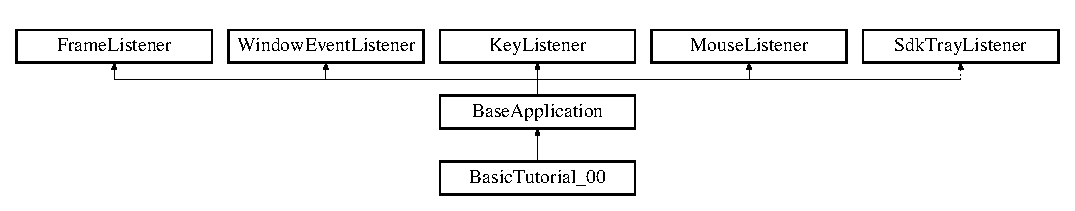
\includegraphics[height=2.382979cm]{class_base_application}
\end{center}
\end{figure}
\subsection*{Public Member Functions}
\begin{DoxyCompactItemize}
\item 
\mbox{\hyperlink{class_base_application_a7c897f08816cc064568ae1ec71026719}{Base\+Application}} (void)
\item 
virtual \mbox{\hyperlink{class_base_application_a48e1966307d5ef8f6cbf8b6e980ad652}{$\sim$\+Base\+Application}} (void)
\item 
virtual void \mbox{\hyperlink{class_base_application_a8a14a65a29118dd75173aa68678a05e1}{go}} (void)
\end{DoxyCompactItemize}
\subsection*{Protected Member Functions}
\begin{DoxyCompactItemize}
\item 
virtual bool \mbox{\hyperlink{class_base_application_a5853d0e148cb85b0297a6885e1d33a89}{setup}} ()
\item 
virtual bool \mbox{\hyperlink{class_base_application_a62ed46f90e9f82cc810997647a2c587e}{configure}} (void)
\item 
virtual void \mbox{\hyperlink{class_base_application_ad5bc9655041e1849a4c13f444a3712bd}{choose\+Scene\+Manager}} (void)
\item 
virtual void \mbox{\hyperlink{class_base_application_afa9d51527763cf9aee9cd4e1b1039d55}{create\+Camera}} (void)
\item 
virtual void \mbox{\hyperlink{class_base_application_aff6fd9ff1ff0978cc68f19dd65be4778}{create\+Frame\+Listener}} (void)
\item 
virtual void \mbox{\hyperlink{class_base_application_aa97beeb4059b17d0ec22eae33286ec2d}{create\+Scene}} (void)=0
\item 
virtual void \mbox{\hyperlink{class_base_application_a365146059b25391fe400f5fdb94f011e}{destroy\+Scene}} (void)
\item 
virtual void \mbox{\hyperlink{class_base_application_a1f8f6730cae6ec769d8730b1af48486e}{create\+Viewports}} (void)
\item 
virtual void \mbox{\hyperlink{class_base_application_ae27301702f1e5de64619a39b1929f1f9}{setup\+Resources}} (void)
\item 
virtual void \mbox{\hyperlink{class_base_application_a9b77972f0f747a61e1f8ceba2ad47641}{create\+Resource\+Listener}} (void)
\item 
virtual void \mbox{\hyperlink{class_base_application_aaeb764e637dd87601a81a80156659d88}{load\+Resources}} (void)
\item 
virtual bool \mbox{\hyperlink{class_base_application_a03912a0f38b38fede7f08a2571e8fc56}{frame\+Rendering\+Queued}} (const Ogre\+::\+Frame\+Event \&evt)
\item 
virtual bool \mbox{\hyperlink{class_base_application_acfa977f04e435f18018ece805c1277ec}{key\+Pressed}} (const O\+I\+S\+::\+Key\+Event \&arg)
\item 
virtual bool \mbox{\hyperlink{class_base_application_aba5c7c9dea7a0efc58b89310bae547e5}{key\+Released}} (const O\+I\+S\+::\+Key\+Event \&arg)
\item 
virtual bool \mbox{\hyperlink{class_base_application_a126e59cb246b061e51eb6ce06a2ee8f4}{mouse\+Moved}} (const O\+I\+S\+::\+Mouse\+Event \&arg)
\item 
virtual bool \mbox{\hyperlink{class_base_application_a9255dfc1eabefd11c474ec45a6622504}{mouse\+Pressed}} (const O\+I\+S\+::\+Mouse\+Event \&arg, O\+I\+S\+::\+Mouse\+Button\+ID id)
\item 
virtual bool \mbox{\hyperlink{class_base_application_aa102c5859c14c0690c749994a446b53d}{mouse\+Released}} (const O\+I\+S\+::\+Mouse\+Event \&arg, O\+I\+S\+::\+Mouse\+Button\+ID id)
\item 
virtual void \mbox{\hyperlink{class_base_application_afacf8a797588592ef0abbad593f10cfa}{window\+Resized}} (Ogre\+::\+Render\+Window $\ast$rw)
\item 
virtual void \mbox{\hyperlink{class_base_application_ae0e37ac54a31ff6e51d58c7654ad1b90}{window\+Closed}} (Ogre\+::\+Render\+Window $\ast$rw)
\end{DoxyCompactItemize}
\subsection*{Protected Attributes}
\begin{DoxyCompactItemize}
\item 
Ogre\+::\+Root $\ast$ \mbox{\hyperlink{class_base_application_add84ba707dc6c57e6283f214b1274110}{m\+Root}}
\item 
Ogre\+::\+Camera $\ast$ \mbox{\hyperlink{class_base_application_a3829c6b12afe911e97e6b4524b33a38b}{m\+Camera}}
\item 
Ogre\+::\+Scene\+Manager $\ast$ \mbox{\hyperlink{class_base_application_a8a7684f4f9a57ed3089048ad1a913b2d}{m\+Scene\+Mgr}}
\item 
Ogre\+::\+Render\+Window $\ast$ \mbox{\hyperlink{class_base_application_ac5d8e9c81e036897bc82f81eff8c570f}{m\+Window}}
\item 
Ogre\+::\+String \mbox{\hyperlink{class_base_application_a765e0df01c141a16df3178ab4f17afe6}{m\+Resources\+Cfg}}
\item 
Ogre\+::\+String \mbox{\hyperlink{class_base_application_a04f2fe47fa164fd78d986dc0df70b7fb}{m\+Plugins\+Cfg}}
\item 
Ogre\+Bites\+::\+Sdk\+Tray\+Manager $\ast$ \mbox{\hyperlink{class_base_application_a7faa397f4f4861ee8c361a01e90b4416}{m\+Tray\+Mgr}}
\item 
Ogre\+Bites\+::\+Sdk\+Camera\+Man $\ast$ \mbox{\hyperlink{class_base_application_a9ae38dea6316058549151fff66a91fcd}{m\+Camera\+Man}}
\item 
Ogre\+Bites\+::\+Params\+Panel $\ast$ \mbox{\hyperlink{class_base_application_a6a11054ca61efdf558e0ff1b2de43a12}{m\+Details\+Panel}}
\item 
bool \mbox{\hyperlink{class_base_application_ac7e861799862cb645f1d78b170aef80d}{m\+Cursor\+Was\+Visible}}
\item 
bool \mbox{\hyperlink{class_base_application_a755f26d3a9915aaf830750d877e39d86}{m\+Shut\+Down}}
\item 
O\+I\+S\+::\+Input\+Manager $\ast$ \mbox{\hyperlink{class_base_application_abc9503c8462e225b5d0d55c952d9e4a9}{m\+Input\+Manager}}
\item 
O\+I\+S\+::\+Mouse $\ast$ \mbox{\hyperlink{class_base_application_add9b97fbe64da2814d3af113bac58c43}{m\+Mouse}}
\item 
O\+I\+S\+::\+Keyboard $\ast$ \mbox{\hyperlink{class_base_application_a9d6e19cf50c47379fbaae55bff28079c}{m\+Keyboard}}
\end{DoxyCompactItemize}


\subsection{Constructor \& Destructor Documentation}
\mbox{\Hypertarget{class_base_application_a7c897f08816cc064568ae1ec71026719}\label{class_base_application_a7c897f08816cc064568ae1ec71026719}} 
\index{Base\+Application@{Base\+Application}!Base\+Application@{Base\+Application}}
\index{Base\+Application@{Base\+Application}!Base\+Application@{Base\+Application}}
\subsubsection{\texorpdfstring{Base\+Application()}{BaseApplication()}}
{\footnotesize\ttfamily Base\+Application\+::\+Base\+Application (\begin{DoxyParamCaption}\item[{void}]{ }\end{DoxyParamCaption})}

\mbox{\Hypertarget{class_base_application_a48e1966307d5ef8f6cbf8b6e980ad652}\label{class_base_application_a48e1966307d5ef8f6cbf8b6e980ad652}} 
\index{Base\+Application@{Base\+Application}!````~Base\+Application@{$\sim$\+Base\+Application}}
\index{````~Base\+Application@{$\sim$\+Base\+Application}!Base\+Application@{Base\+Application}}
\subsubsection{\texorpdfstring{$\sim$\+Base\+Application()}{~BaseApplication()}}
{\footnotesize\ttfamily Base\+Application\+::$\sim$\+Base\+Application (\begin{DoxyParamCaption}\item[{void}]{ }\end{DoxyParamCaption})\hspace{0.3cm}{\ttfamily [virtual]}}



\subsection{Member Function Documentation}
\mbox{\Hypertarget{class_base_application_ad5bc9655041e1849a4c13f444a3712bd}\label{class_base_application_ad5bc9655041e1849a4c13f444a3712bd}} 
\index{Base\+Application@{Base\+Application}!choose\+Scene\+Manager@{choose\+Scene\+Manager}}
\index{choose\+Scene\+Manager@{choose\+Scene\+Manager}!Base\+Application@{Base\+Application}}
\subsubsection{\texorpdfstring{choose\+Scene\+Manager()}{chooseSceneManager()}}
{\footnotesize\ttfamily void Base\+Application\+::choose\+Scene\+Manager (\begin{DoxyParamCaption}\item[{void}]{ }\end{DoxyParamCaption})\hspace{0.3cm}{\ttfamily [protected]}, {\ttfamily [virtual]}}



Reimplemented in \mbox{\hyperlink{class_basic_tutorial__00_aba97a29d983586d2dc8e108d3bccf721}{Basic\+Tutorial\+\_\+00}}.

\mbox{\Hypertarget{class_base_application_a62ed46f90e9f82cc810997647a2c587e}\label{class_base_application_a62ed46f90e9f82cc810997647a2c587e}} 
\index{Base\+Application@{Base\+Application}!configure@{configure}}
\index{configure@{configure}!Base\+Application@{Base\+Application}}
\subsubsection{\texorpdfstring{configure()}{configure()}}
{\footnotesize\ttfamily bool Base\+Application\+::configure (\begin{DoxyParamCaption}\item[{void}]{ }\end{DoxyParamCaption})\hspace{0.3cm}{\ttfamily [protected]}, {\ttfamily [virtual]}}

\mbox{\Hypertarget{class_base_application_afa9d51527763cf9aee9cd4e1b1039d55}\label{class_base_application_afa9d51527763cf9aee9cd4e1b1039d55}} 
\index{Base\+Application@{Base\+Application}!create\+Camera@{create\+Camera}}
\index{create\+Camera@{create\+Camera}!Base\+Application@{Base\+Application}}
\subsubsection{\texorpdfstring{create\+Camera()}{createCamera()}}
{\footnotesize\ttfamily void Base\+Application\+::create\+Camera (\begin{DoxyParamCaption}\item[{void}]{ }\end{DoxyParamCaption})\hspace{0.3cm}{\ttfamily [protected]}, {\ttfamily [virtual]}}



Reimplemented in \mbox{\hyperlink{class_basic_tutorial__00_a1bf709417d654dffc2ea10987412b912}{Basic\+Tutorial\+\_\+00}}.

\mbox{\Hypertarget{class_base_application_aff6fd9ff1ff0978cc68f19dd65be4778}\label{class_base_application_aff6fd9ff1ff0978cc68f19dd65be4778}} 
\index{Base\+Application@{Base\+Application}!create\+Frame\+Listener@{create\+Frame\+Listener}}
\index{create\+Frame\+Listener@{create\+Frame\+Listener}!Base\+Application@{Base\+Application}}
\subsubsection{\texorpdfstring{create\+Frame\+Listener()}{createFrameListener()}}
{\footnotesize\ttfamily void Base\+Application\+::create\+Frame\+Listener (\begin{DoxyParamCaption}\item[{void}]{ }\end{DoxyParamCaption})\hspace{0.3cm}{\ttfamily [protected]}, {\ttfamily [virtual]}}

\mbox{\Hypertarget{class_base_application_a9b77972f0f747a61e1f8ceba2ad47641}\label{class_base_application_a9b77972f0f747a61e1f8ceba2ad47641}} 
\index{Base\+Application@{Base\+Application}!create\+Resource\+Listener@{create\+Resource\+Listener}}
\index{create\+Resource\+Listener@{create\+Resource\+Listener}!Base\+Application@{Base\+Application}}
\subsubsection{\texorpdfstring{create\+Resource\+Listener()}{createResourceListener()}}
{\footnotesize\ttfamily void Base\+Application\+::create\+Resource\+Listener (\begin{DoxyParamCaption}\item[{void}]{ }\end{DoxyParamCaption})\hspace{0.3cm}{\ttfamily [protected]}, {\ttfamily [virtual]}}

\mbox{\Hypertarget{class_base_application_aa97beeb4059b17d0ec22eae33286ec2d}\label{class_base_application_aa97beeb4059b17d0ec22eae33286ec2d}} 
\index{Base\+Application@{Base\+Application}!create\+Scene@{create\+Scene}}
\index{create\+Scene@{create\+Scene}!Base\+Application@{Base\+Application}}
\subsubsection{\texorpdfstring{create\+Scene()}{createScene()}}
{\footnotesize\ttfamily virtual void Base\+Application\+::create\+Scene (\begin{DoxyParamCaption}\item[{void}]{ }\end{DoxyParamCaption})\hspace{0.3cm}{\ttfamily [protected]}, {\ttfamily [pure virtual]}}



Implemented in \mbox{\hyperlink{class_basic_tutorial__00_a15a3d4673724ec99077ce992f996a550}{Basic\+Tutorial\+\_\+00}}.

\mbox{\Hypertarget{class_base_application_a1f8f6730cae6ec769d8730b1af48486e}\label{class_base_application_a1f8f6730cae6ec769d8730b1af48486e}} 
\index{Base\+Application@{Base\+Application}!create\+Viewports@{create\+Viewports}}
\index{create\+Viewports@{create\+Viewports}!Base\+Application@{Base\+Application}}
\subsubsection{\texorpdfstring{create\+Viewports()}{createViewports()}}
{\footnotesize\ttfamily void Base\+Application\+::create\+Viewports (\begin{DoxyParamCaption}\item[{void}]{ }\end{DoxyParamCaption})\hspace{0.3cm}{\ttfamily [protected]}, {\ttfamily [virtual]}}



Reimplemented in \mbox{\hyperlink{class_basic_tutorial__00_adc2454d9f8226e0958ecf702f355846e}{Basic\+Tutorial\+\_\+00}}.

\mbox{\Hypertarget{class_base_application_a365146059b25391fe400f5fdb94f011e}\label{class_base_application_a365146059b25391fe400f5fdb94f011e}} 
\index{Base\+Application@{Base\+Application}!destroy\+Scene@{destroy\+Scene}}
\index{destroy\+Scene@{destroy\+Scene}!Base\+Application@{Base\+Application}}
\subsubsection{\texorpdfstring{destroy\+Scene()}{destroyScene()}}
{\footnotesize\ttfamily void Base\+Application\+::destroy\+Scene (\begin{DoxyParamCaption}\item[{void}]{ }\end{DoxyParamCaption})\hspace{0.3cm}{\ttfamily [protected]}, {\ttfamily [virtual]}}

\mbox{\Hypertarget{class_base_application_a03912a0f38b38fede7f08a2571e8fc56}\label{class_base_application_a03912a0f38b38fede7f08a2571e8fc56}} 
\index{Base\+Application@{Base\+Application}!frame\+Rendering\+Queued@{frame\+Rendering\+Queued}}
\index{frame\+Rendering\+Queued@{frame\+Rendering\+Queued}!Base\+Application@{Base\+Application}}
\subsubsection{\texorpdfstring{frame\+Rendering\+Queued()}{frameRenderingQueued()}}
{\footnotesize\ttfamily bool Base\+Application\+::frame\+Rendering\+Queued (\begin{DoxyParamCaption}\item[{const Ogre\+::\+Frame\+Event \&}]{evt }\end{DoxyParamCaption})\hspace{0.3cm}{\ttfamily [protected]}, {\ttfamily [virtual]}}

\mbox{\Hypertarget{class_base_application_a8a14a65a29118dd75173aa68678a05e1}\label{class_base_application_a8a14a65a29118dd75173aa68678a05e1}} 
\index{Base\+Application@{Base\+Application}!go@{go}}
\index{go@{go}!Base\+Application@{Base\+Application}}
\subsubsection{\texorpdfstring{go()}{go()}}
{\footnotesize\ttfamily void Base\+Application\+::go (\begin{DoxyParamCaption}\item[{void}]{ }\end{DoxyParamCaption})\hspace{0.3cm}{\ttfamily [virtual]}}

\mbox{\Hypertarget{class_base_application_acfa977f04e435f18018ece805c1277ec}\label{class_base_application_acfa977f04e435f18018ece805c1277ec}} 
\index{Base\+Application@{Base\+Application}!key\+Pressed@{key\+Pressed}}
\index{key\+Pressed@{key\+Pressed}!Base\+Application@{Base\+Application}}
\subsubsection{\texorpdfstring{key\+Pressed()}{keyPressed()}}
{\footnotesize\ttfamily bool Base\+Application\+::key\+Pressed (\begin{DoxyParamCaption}\item[{const O\+I\+S\+::\+Key\+Event \&}]{arg }\end{DoxyParamCaption})\hspace{0.3cm}{\ttfamily [protected]}, {\ttfamily [virtual]}}



Reimplemented in \mbox{\hyperlink{class_basic_tutorial__00_adc1a0b32d78b1980b3ee51a1b1e1e69b}{Basic\+Tutorial\+\_\+00}}.

\mbox{\Hypertarget{class_base_application_aba5c7c9dea7a0efc58b89310bae547e5}\label{class_base_application_aba5c7c9dea7a0efc58b89310bae547e5}} 
\index{Base\+Application@{Base\+Application}!key\+Released@{key\+Released}}
\index{key\+Released@{key\+Released}!Base\+Application@{Base\+Application}}
\subsubsection{\texorpdfstring{key\+Released()}{keyReleased()}}
{\footnotesize\ttfamily bool Base\+Application\+::key\+Released (\begin{DoxyParamCaption}\item[{const O\+I\+S\+::\+Key\+Event \&}]{arg }\end{DoxyParamCaption})\hspace{0.3cm}{\ttfamily [protected]}, {\ttfamily [virtual]}}



Reimplemented in \mbox{\hyperlink{class_basic_tutorial__00_aacca7a0a2a5a0e0d007b9c6c30b4941b}{Basic\+Tutorial\+\_\+00}}.

\mbox{\Hypertarget{class_base_application_aaeb764e637dd87601a81a80156659d88}\label{class_base_application_aaeb764e637dd87601a81a80156659d88}} 
\index{Base\+Application@{Base\+Application}!load\+Resources@{load\+Resources}}
\index{load\+Resources@{load\+Resources}!Base\+Application@{Base\+Application}}
\subsubsection{\texorpdfstring{load\+Resources()}{loadResources()}}
{\footnotesize\ttfamily void Base\+Application\+::load\+Resources (\begin{DoxyParamCaption}\item[{void}]{ }\end{DoxyParamCaption})\hspace{0.3cm}{\ttfamily [protected]}, {\ttfamily [virtual]}}

\mbox{\Hypertarget{class_base_application_a126e59cb246b061e51eb6ce06a2ee8f4}\label{class_base_application_a126e59cb246b061e51eb6ce06a2ee8f4}} 
\index{Base\+Application@{Base\+Application}!mouse\+Moved@{mouse\+Moved}}
\index{mouse\+Moved@{mouse\+Moved}!Base\+Application@{Base\+Application}}
\subsubsection{\texorpdfstring{mouse\+Moved()}{mouseMoved()}}
{\footnotesize\ttfamily bool Base\+Application\+::mouse\+Moved (\begin{DoxyParamCaption}\item[{const O\+I\+S\+::\+Mouse\+Event \&}]{arg }\end{DoxyParamCaption})\hspace{0.3cm}{\ttfamily [protected]}, {\ttfamily [virtual]}}

\mbox{\Hypertarget{class_base_application_a9255dfc1eabefd11c474ec45a6622504}\label{class_base_application_a9255dfc1eabefd11c474ec45a6622504}} 
\index{Base\+Application@{Base\+Application}!mouse\+Pressed@{mouse\+Pressed}}
\index{mouse\+Pressed@{mouse\+Pressed}!Base\+Application@{Base\+Application}}
\subsubsection{\texorpdfstring{mouse\+Pressed()}{mousePressed()}}
{\footnotesize\ttfamily bool Base\+Application\+::mouse\+Pressed (\begin{DoxyParamCaption}\item[{const O\+I\+S\+::\+Mouse\+Event \&}]{arg,  }\item[{O\+I\+S\+::\+Mouse\+Button\+ID}]{id }\end{DoxyParamCaption})\hspace{0.3cm}{\ttfamily [protected]}, {\ttfamily [virtual]}}

\mbox{\Hypertarget{class_base_application_aa102c5859c14c0690c749994a446b53d}\label{class_base_application_aa102c5859c14c0690c749994a446b53d}} 
\index{Base\+Application@{Base\+Application}!mouse\+Released@{mouse\+Released}}
\index{mouse\+Released@{mouse\+Released}!Base\+Application@{Base\+Application}}
\subsubsection{\texorpdfstring{mouse\+Released()}{mouseReleased()}}
{\footnotesize\ttfamily bool Base\+Application\+::mouse\+Released (\begin{DoxyParamCaption}\item[{const O\+I\+S\+::\+Mouse\+Event \&}]{arg,  }\item[{O\+I\+S\+::\+Mouse\+Button\+ID}]{id }\end{DoxyParamCaption})\hspace{0.3cm}{\ttfamily [protected]}, {\ttfamily [virtual]}}

\mbox{\Hypertarget{class_base_application_a5853d0e148cb85b0297a6885e1d33a89}\label{class_base_application_a5853d0e148cb85b0297a6885e1d33a89}} 
\index{Base\+Application@{Base\+Application}!setup@{setup}}
\index{setup@{setup}!Base\+Application@{Base\+Application}}
\subsubsection{\texorpdfstring{setup()}{setup()}}
{\footnotesize\ttfamily bool Base\+Application\+::setup (\begin{DoxyParamCaption}\item[{void}]{ }\end{DoxyParamCaption})\hspace{0.3cm}{\ttfamily [protected]}, {\ttfamily [virtual]}}

\mbox{\Hypertarget{class_base_application_ae27301702f1e5de64619a39b1929f1f9}\label{class_base_application_ae27301702f1e5de64619a39b1929f1f9}} 
\index{Base\+Application@{Base\+Application}!setup\+Resources@{setup\+Resources}}
\index{setup\+Resources@{setup\+Resources}!Base\+Application@{Base\+Application}}
\subsubsection{\texorpdfstring{setup\+Resources()}{setupResources()}}
{\footnotesize\ttfamily void Base\+Application\+::setup\+Resources (\begin{DoxyParamCaption}\item[{void}]{ }\end{DoxyParamCaption})\hspace{0.3cm}{\ttfamily [protected]}, {\ttfamily [virtual]}}

\mbox{\Hypertarget{class_base_application_ae0e37ac54a31ff6e51d58c7654ad1b90}\label{class_base_application_ae0e37ac54a31ff6e51d58c7654ad1b90}} 
\index{Base\+Application@{Base\+Application}!window\+Closed@{window\+Closed}}
\index{window\+Closed@{window\+Closed}!Base\+Application@{Base\+Application}}
\subsubsection{\texorpdfstring{window\+Closed()}{windowClosed()}}
{\footnotesize\ttfamily void Base\+Application\+::window\+Closed (\begin{DoxyParamCaption}\item[{Ogre\+::\+Render\+Window $\ast$}]{rw }\end{DoxyParamCaption})\hspace{0.3cm}{\ttfamily [protected]}, {\ttfamily [virtual]}}

\mbox{\Hypertarget{class_base_application_afacf8a797588592ef0abbad593f10cfa}\label{class_base_application_afacf8a797588592ef0abbad593f10cfa}} 
\index{Base\+Application@{Base\+Application}!window\+Resized@{window\+Resized}}
\index{window\+Resized@{window\+Resized}!Base\+Application@{Base\+Application}}
\subsubsection{\texorpdfstring{window\+Resized()}{windowResized()}}
{\footnotesize\ttfamily void Base\+Application\+::window\+Resized (\begin{DoxyParamCaption}\item[{Ogre\+::\+Render\+Window $\ast$}]{rw }\end{DoxyParamCaption})\hspace{0.3cm}{\ttfamily [protected]}, {\ttfamily [virtual]}}



\subsection{Member Data Documentation}
\mbox{\Hypertarget{class_base_application_a3829c6b12afe911e97e6b4524b33a38b}\label{class_base_application_a3829c6b12afe911e97e6b4524b33a38b}} 
\index{Base\+Application@{Base\+Application}!m\+Camera@{m\+Camera}}
\index{m\+Camera@{m\+Camera}!Base\+Application@{Base\+Application}}
\subsubsection{\texorpdfstring{m\+Camera}{mCamera}}
{\footnotesize\ttfamily Ogre\+::\+Camera$\ast$ Base\+Application\+::m\+Camera\hspace{0.3cm}{\ttfamily [protected]}}

\mbox{\Hypertarget{class_base_application_a9ae38dea6316058549151fff66a91fcd}\label{class_base_application_a9ae38dea6316058549151fff66a91fcd}} 
\index{Base\+Application@{Base\+Application}!m\+Camera\+Man@{m\+Camera\+Man}}
\index{m\+Camera\+Man@{m\+Camera\+Man}!Base\+Application@{Base\+Application}}
\subsubsection{\texorpdfstring{m\+Camera\+Man}{mCameraMan}}
{\footnotesize\ttfamily Ogre\+Bites\+::\+Sdk\+Camera\+Man$\ast$ Base\+Application\+::m\+Camera\+Man\hspace{0.3cm}{\ttfamily [protected]}}

\mbox{\Hypertarget{class_base_application_ac7e861799862cb645f1d78b170aef80d}\label{class_base_application_ac7e861799862cb645f1d78b170aef80d}} 
\index{Base\+Application@{Base\+Application}!m\+Cursor\+Was\+Visible@{m\+Cursor\+Was\+Visible}}
\index{m\+Cursor\+Was\+Visible@{m\+Cursor\+Was\+Visible}!Base\+Application@{Base\+Application}}
\subsubsection{\texorpdfstring{m\+Cursor\+Was\+Visible}{mCursorWasVisible}}
{\footnotesize\ttfamily bool Base\+Application\+::m\+Cursor\+Was\+Visible\hspace{0.3cm}{\ttfamily [protected]}}

\mbox{\Hypertarget{class_base_application_a6a11054ca61efdf558e0ff1b2de43a12}\label{class_base_application_a6a11054ca61efdf558e0ff1b2de43a12}} 
\index{Base\+Application@{Base\+Application}!m\+Details\+Panel@{m\+Details\+Panel}}
\index{m\+Details\+Panel@{m\+Details\+Panel}!Base\+Application@{Base\+Application}}
\subsubsection{\texorpdfstring{m\+Details\+Panel}{mDetailsPanel}}
{\footnotesize\ttfamily Ogre\+Bites\+::\+Params\+Panel$\ast$ Base\+Application\+::m\+Details\+Panel\hspace{0.3cm}{\ttfamily [protected]}}

\mbox{\Hypertarget{class_base_application_abc9503c8462e225b5d0d55c952d9e4a9}\label{class_base_application_abc9503c8462e225b5d0d55c952d9e4a9}} 
\index{Base\+Application@{Base\+Application}!m\+Input\+Manager@{m\+Input\+Manager}}
\index{m\+Input\+Manager@{m\+Input\+Manager}!Base\+Application@{Base\+Application}}
\subsubsection{\texorpdfstring{m\+Input\+Manager}{mInputManager}}
{\footnotesize\ttfamily O\+I\+S\+::\+Input\+Manager$\ast$ Base\+Application\+::m\+Input\+Manager\hspace{0.3cm}{\ttfamily [protected]}}

\mbox{\Hypertarget{class_base_application_a9d6e19cf50c47379fbaae55bff28079c}\label{class_base_application_a9d6e19cf50c47379fbaae55bff28079c}} 
\index{Base\+Application@{Base\+Application}!m\+Keyboard@{m\+Keyboard}}
\index{m\+Keyboard@{m\+Keyboard}!Base\+Application@{Base\+Application}}
\subsubsection{\texorpdfstring{m\+Keyboard}{mKeyboard}}
{\footnotesize\ttfamily O\+I\+S\+::\+Keyboard$\ast$ Base\+Application\+::m\+Keyboard\hspace{0.3cm}{\ttfamily [protected]}}

\mbox{\Hypertarget{class_base_application_add9b97fbe64da2814d3af113bac58c43}\label{class_base_application_add9b97fbe64da2814d3af113bac58c43}} 
\index{Base\+Application@{Base\+Application}!m\+Mouse@{m\+Mouse}}
\index{m\+Mouse@{m\+Mouse}!Base\+Application@{Base\+Application}}
\subsubsection{\texorpdfstring{m\+Mouse}{mMouse}}
{\footnotesize\ttfamily O\+I\+S\+::\+Mouse$\ast$ Base\+Application\+::m\+Mouse\hspace{0.3cm}{\ttfamily [protected]}}

\mbox{\Hypertarget{class_base_application_a04f2fe47fa164fd78d986dc0df70b7fb}\label{class_base_application_a04f2fe47fa164fd78d986dc0df70b7fb}} 
\index{Base\+Application@{Base\+Application}!m\+Plugins\+Cfg@{m\+Plugins\+Cfg}}
\index{m\+Plugins\+Cfg@{m\+Plugins\+Cfg}!Base\+Application@{Base\+Application}}
\subsubsection{\texorpdfstring{m\+Plugins\+Cfg}{mPluginsCfg}}
{\footnotesize\ttfamily Ogre\+::\+String Base\+Application\+::m\+Plugins\+Cfg\hspace{0.3cm}{\ttfamily [protected]}}

\mbox{\Hypertarget{class_base_application_a765e0df01c141a16df3178ab4f17afe6}\label{class_base_application_a765e0df01c141a16df3178ab4f17afe6}} 
\index{Base\+Application@{Base\+Application}!m\+Resources\+Cfg@{m\+Resources\+Cfg}}
\index{m\+Resources\+Cfg@{m\+Resources\+Cfg}!Base\+Application@{Base\+Application}}
\subsubsection{\texorpdfstring{m\+Resources\+Cfg}{mResourcesCfg}}
{\footnotesize\ttfamily Ogre\+::\+String Base\+Application\+::m\+Resources\+Cfg\hspace{0.3cm}{\ttfamily [protected]}}

\mbox{\Hypertarget{class_base_application_add84ba707dc6c57e6283f214b1274110}\label{class_base_application_add84ba707dc6c57e6283f214b1274110}} 
\index{Base\+Application@{Base\+Application}!m\+Root@{m\+Root}}
\index{m\+Root@{m\+Root}!Base\+Application@{Base\+Application}}
\subsubsection{\texorpdfstring{m\+Root}{mRoot}}
{\footnotesize\ttfamily Ogre\+::\+Root$\ast$ Base\+Application\+::m\+Root\hspace{0.3cm}{\ttfamily [protected]}}

\mbox{\Hypertarget{class_base_application_a8a7684f4f9a57ed3089048ad1a913b2d}\label{class_base_application_a8a7684f4f9a57ed3089048ad1a913b2d}} 
\index{Base\+Application@{Base\+Application}!m\+Scene\+Mgr@{m\+Scene\+Mgr}}
\index{m\+Scene\+Mgr@{m\+Scene\+Mgr}!Base\+Application@{Base\+Application}}
\subsubsection{\texorpdfstring{m\+Scene\+Mgr}{mSceneMgr}}
{\footnotesize\ttfamily Ogre\+::\+Scene\+Manager$\ast$ Base\+Application\+::m\+Scene\+Mgr\hspace{0.3cm}{\ttfamily [protected]}}

\mbox{\Hypertarget{class_base_application_a755f26d3a9915aaf830750d877e39d86}\label{class_base_application_a755f26d3a9915aaf830750d877e39d86}} 
\index{Base\+Application@{Base\+Application}!m\+Shut\+Down@{m\+Shut\+Down}}
\index{m\+Shut\+Down@{m\+Shut\+Down}!Base\+Application@{Base\+Application}}
\subsubsection{\texorpdfstring{m\+Shut\+Down}{mShutDown}}
{\footnotesize\ttfamily bool Base\+Application\+::m\+Shut\+Down\hspace{0.3cm}{\ttfamily [protected]}}

\mbox{\Hypertarget{class_base_application_a7faa397f4f4861ee8c361a01e90b4416}\label{class_base_application_a7faa397f4f4861ee8c361a01e90b4416}} 
\index{Base\+Application@{Base\+Application}!m\+Tray\+Mgr@{m\+Tray\+Mgr}}
\index{m\+Tray\+Mgr@{m\+Tray\+Mgr}!Base\+Application@{Base\+Application}}
\subsubsection{\texorpdfstring{m\+Tray\+Mgr}{mTrayMgr}}
{\footnotesize\ttfamily Ogre\+Bites\+::\+Sdk\+Tray\+Manager$\ast$ Base\+Application\+::m\+Tray\+Mgr\hspace{0.3cm}{\ttfamily [protected]}}

\mbox{\Hypertarget{class_base_application_ac5d8e9c81e036897bc82f81eff8c570f}\label{class_base_application_ac5d8e9c81e036897bc82f81eff8c570f}} 
\index{Base\+Application@{Base\+Application}!m\+Window@{m\+Window}}
\index{m\+Window@{m\+Window}!Base\+Application@{Base\+Application}}
\subsubsection{\texorpdfstring{m\+Window}{mWindow}}
{\footnotesize\ttfamily Ogre\+::\+Render\+Window$\ast$ Base\+Application\+::m\+Window\hspace{0.3cm}{\ttfamily [protected]}}



The documentation for this class was generated from the following files\+:\begin{DoxyCompactItemize}
\item 
\mbox{\hyperlink{_base_application_8h}{Base\+Application.\+h}}\item 
\mbox{\hyperlink{_base_application_8cpp}{Base\+Application.\+cpp}}\end{DoxyCompactItemize}

\hypertarget{class_basic_tutorial__00}{}\section{Basic\+Tutorial\+\_\+00 Class Reference}
\label{class_basic_tutorial__00}\index{Basic\+Tutorial\+\_\+00@{Basic\+Tutorial\+\_\+00}}


3D Game Programming ~\newline
My Name\+: Chien-\/\+Yao Huang ~\newline
My ID\+: 0656651 ~\newline
My Email\+: \href{mailto:hk850522@gmail.com}{\tt hk850522@gmail.\+com} ~\newline
 Date\+: 2018/09/20  




{\ttfamily \#include $<$Tutorial\+Application.\+h$>$}

Inheritance diagram for Basic\+Tutorial\+\_\+00\+:\begin{figure}[H]
\begin{center}
\leavevmode
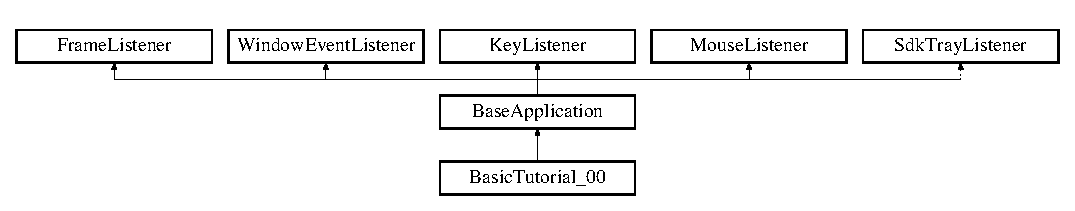
\includegraphics[height=2.382979cm]{class_basic_tutorial__00}
\end{center}
\end{figure}
\subsection*{Public Member Functions}
\begin{DoxyCompactItemize}
\item 
\mbox{\hyperlink{class_basic_tutorial__00_a6b55068822076b28e7819b1878e95684}{Basic\+Tutorial\+\_\+00}} (void)
\item 
virtual void \mbox{\hyperlink{class_basic_tutorial__00_aba97a29d983586d2dc8e108d3bccf721}{choose\+Scene\+Manager}} (void)
\item 
virtual void \mbox{\hyperlink{class_basic_tutorial__00_a1bf709417d654dffc2ea10987412b912}{create\+Camera}} (void)
\item 
virtual void \mbox{\hyperlink{class_basic_tutorial__00_adc2454d9f8226e0958ecf702f355846e}{create\+Viewports}} (void)
\item 
virtual void \mbox{\hyperlink{class_basic_tutorial__00_a15a3d4673724ec99077ce992f996a550}{create\+Scene}} (void)
\item 
virtual bool \mbox{\hyperlink{class_basic_tutorial__00_a94e281a96584a25bf57b1c5e73737c81}{frame\+Started}} (const Ogre\+::\+Frame\+Event \&evt)
\end{DoxyCompactItemize}
\subsection*{Protected Member Functions}
\begin{DoxyCompactItemize}
\item 
void \mbox{\hyperlink{class_basic_tutorial__00_a6d4684502f2f7b2cf628a975d7750d8e}{create\+Viewport\+\_\+00}} (void)
\begin{DoxyCompactList}\small\item\em Create a viewport. \end{DoxyCompactList}\item 
void \mbox{\hyperlink{class_basic_tutorial__00_a2801a2f0d91d80b471da48344d2ccccf}{create\+Viewport\+\_\+01}} (void)
\begin{DoxyCompactList}\small\item\em Create a viewport. \end{DoxyCompactList}\item 
void \mbox{\hyperlink{class_basic_tutorial__00_a3479c50dbf8dc06a7ea77014eb94c6e7}{create\+Camera\+\_\+00}} ()
\begin{DoxyCompactList}\small\item\em Create a camera. \end{DoxyCompactList}\item 
void \mbox{\hyperlink{class_basic_tutorial__00_a8745a127adeb69fa769f832fd41412c0}{create\+Camera\+\_\+01}} ()
\begin{DoxyCompactList}\small\item\em Create a camera. \end{DoxyCompactList}\item 
void \mbox{\hyperlink{class_basic_tutorial__00_aa84173e509858146cbfb98274c1ef56e}{create\+Scene\+\_\+00}} ()
\begin{DoxyCompactList}\small\item\em Create the main scene. \end{DoxyCompactList}\item 
void \mbox{\hyperlink{class_basic_tutorial__00_aad14e1ca565797c4b7dcff31bc0e1494}{create\+Scene\+\_\+01}} ()
\begin{DoxyCompactList}\small\item\em Create the second scene. \end{DoxyCompactList}\item 
bool \mbox{\hyperlink{class_basic_tutorial__00_adc1a0b32d78b1980b3ee51a1b1e1e69b}{key\+Pressed}} (const O\+I\+S\+::\+Key\+Event \&arg)
\item 
bool \mbox{\hyperlink{class_basic_tutorial__00_aacca7a0a2a5a0e0d007b9c6c30b4941b}{key\+Released}} (const O\+I\+S\+::\+Key\+Event \&arg)
\item 
void \mbox{\hyperlink{class_basic_tutorial__00_a6ee6fde3630cd34a586432ba0f7547d7}{change\+Viewport}} ()
\end{DoxyCompactItemize}
\subsection*{Protected Attributes}
\begin{DoxyCompactItemize}
\item 
Ogre\+::\+Viewport $\ast$ \mbox{\hyperlink{class_basic_tutorial__00_a6676a92b50e9b43634d4c66488537b73}{m\+Viewport\+Arr}} \mbox{[}8\mbox{]}
\item 
Ogre\+::\+Camera $\ast$ \mbox{\hyperlink{class_basic_tutorial__00_af8d457d912286a98c0975c52d4faf910}{m\+Camera\+Arr}} \mbox{[}8\mbox{]}
\item 
Ogre\+::\+Scene\+Manager $\ast$ \mbox{\hyperlink{class_basic_tutorial__00_a603779b6087698c57b7989e16d8a9b93}{m\+Scene\+Mgr\+Arr}} \mbox{[}8\mbox{]}
\item 
Ogre\+Bites\+::\+Sdk\+Camera\+Man $\ast$ \mbox{\hyperlink{class_basic_tutorial__00_a700c07f924c71e9fa1885a46f599d934}{m\+Camera\+Man\+Arr}} \mbox{[}8\mbox{]}
\item 
bool \mbox{\hyperlink{class_basic_tutorial__00_a0d974de1a6955553775aa06d1df374be}{play\+Anim}}
\item 
bool \mbox{\hyperlink{class_basic_tutorial__00_a26b2c1e7db607fefcfeb65073d3db8ee}{is\+Upward}}
\item 
float \mbox{\hyperlink{class_basic_tutorial__00_a54237e9e69a120912349ee2cadbd3e16}{max\+\_\+height}}
\item 
float \mbox{\hyperlink{class_basic_tutorial__00_a48bd1d1a7035b7edbb90297e2d9f28ec}{min\+\_\+height}}
\item 
float \mbox{\hyperlink{class_basic_tutorial__00_a2448b63a5e8152ac4e6826d7bbf249ca}{max\+\_\+velo}}
\item 
Ogre\+::\+Vector3 \mbox{\hyperlink{class_basic_tutorial__00_a9146709112187aa671a6a6dbe3282556}{velocity}}
\item 
Ogre\+::\+Vector3 \mbox{\hyperlink{class_basic_tutorial__00_ab13a24b7ff14b1cf4da3dbf16bcd0f01}{up\+\_\+acc}}
\item 
Ogre\+::\+Vector3 \mbox{\hyperlink{class_basic_tutorial__00_ac6e8f5f86ae244acb97980b4c31fe370}{down\+\_\+acc}}
\end{DoxyCompactItemize}


\subsection{Detailed Description}
3D Game Programming ~\newline
My Name\+: Chien-\/\+Yao Huang ~\newline
My ID\+: 0656651 ~\newline
My Email\+: \href{mailto:hk850522@gmail.com}{\tt hk850522@gmail.\+com} ~\newline
 Date\+: 2018/09/20 

This is an assignment of 3D Game Programming 

\subsection{Constructor \& Destructor Documentation}
\mbox{\Hypertarget{class_basic_tutorial__00_a6b55068822076b28e7819b1878e95684}\label{class_basic_tutorial__00_a6b55068822076b28e7819b1878e95684}} 
\index{Basic\+Tutorial\+\_\+00@{Basic\+Tutorial\+\_\+00}!Basic\+Tutorial\+\_\+00@{Basic\+Tutorial\+\_\+00}}
\index{Basic\+Tutorial\+\_\+00@{Basic\+Tutorial\+\_\+00}!Basic\+Tutorial\+\_\+00@{Basic\+Tutorial\+\_\+00}}
\subsubsection{\texorpdfstring{Basic\+Tutorial\+\_\+00()}{BasicTutorial\_00()}}
{\footnotesize\ttfamily Basic\+Tutorial\+\_\+00\+::\+Basic\+Tutorial\+\_\+00 (\begin{DoxyParamCaption}\item[{void}]{ }\end{DoxyParamCaption})}



\subsection{Member Function Documentation}
\mbox{\Hypertarget{class_basic_tutorial__00_a6ee6fde3630cd34a586432ba0f7547d7}\label{class_basic_tutorial__00_a6ee6fde3630cd34a586432ba0f7547d7}} 
\index{Basic\+Tutorial\+\_\+00@{Basic\+Tutorial\+\_\+00}!change\+Viewport@{change\+Viewport}}
\index{change\+Viewport@{change\+Viewport}!Basic\+Tutorial\+\_\+00@{Basic\+Tutorial\+\_\+00}}
\subsubsection{\texorpdfstring{change\+Viewport()}{changeViewport()}}
{\footnotesize\ttfamily void Basic\+Tutorial\+\_\+00\+::change\+Viewport (\begin{DoxyParamCaption}{ }\end{DoxyParamCaption})\hspace{0.3cm}{\ttfamily [protected]}}

\mbox{\Hypertarget{class_basic_tutorial__00_aba97a29d983586d2dc8e108d3bccf721}\label{class_basic_tutorial__00_aba97a29d983586d2dc8e108d3bccf721}} 
\index{Basic\+Tutorial\+\_\+00@{Basic\+Tutorial\+\_\+00}!choose\+Scene\+Manager@{choose\+Scene\+Manager}}
\index{choose\+Scene\+Manager@{choose\+Scene\+Manager}!Basic\+Tutorial\+\_\+00@{Basic\+Tutorial\+\_\+00}}
\subsubsection{\texorpdfstring{choose\+Scene\+Manager()}{chooseSceneManager()}}
{\footnotesize\ttfamily void Basic\+Tutorial\+\_\+00\+::choose\+Scene\+Manager (\begin{DoxyParamCaption}\item[{void}]{ }\end{DoxyParamCaption})\hspace{0.3cm}{\ttfamily [virtual]}}



Reimplemented from \mbox{\hyperlink{class_base_application_ad5bc9655041e1849a4c13f444a3712bd}{Base\+Application}}.

\mbox{\Hypertarget{class_basic_tutorial__00_a1bf709417d654dffc2ea10987412b912}\label{class_basic_tutorial__00_a1bf709417d654dffc2ea10987412b912}} 
\index{Basic\+Tutorial\+\_\+00@{Basic\+Tutorial\+\_\+00}!create\+Camera@{create\+Camera}}
\index{create\+Camera@{create\+Camera}!Basic\+Tutorial\+\_\+00@{Basic\+Tutorial\+\_\+00}}
\subsubsection{\texorpdfstring{create\+Camera()}{createCamera()}}
{\footnotesize\ttfamily void Basic\+Tutorial\+\_\+00\+::create\+Camera (\begin{DoxyParamCaption}\item[{void}]{ }\end{DoxyParamCaption})\hspace{0.3cm}{\ttfamily [virtual]}}



Reimplemented from \mbox{\hyperlink{class_base_application_afa9d51527763cf9aee9cd4e1b1039d55}{Base\+Application}}.

\mbox{\Hypertarget{class_basic_tutorial__00_a3479c50dbf8dc06a7ea77014eb94c6e7}\label{class_basic_tutorial__00_a3479c50dbf8dc06a7ea77014eb94c6e7}} 
\index{Basic\+Tutorial\+\_\+00@{Basic\+Tutorial\+\_\+00}!create\+Camera\+\_\+00@{create\+Camera\+\_\+00}}
\index{create\+Camera\+\_\+00@{create\+Camera\+\_\+00}!Basic\+Tutorial\+\_\+00@{Basic\+Tutorial\+\_\+00}}
\subsubsection{\texorpdfstring{create\+Camera\+\_\+00()}{createCamera\_00()}}
{\footnotesize\ttfamily void Basic\+Tutorial\+\_\+00\+::create\+Camera\+\_\+00 (\begin{DoxyParamCaption}\item[{void}]{ }\end{DoxyParamCaption})\hspace{0.3cm}{\ttfamily [protected]}}



Create a camera. 

Create a camera for the main screen.

\begin{DoxyReturn}{Returns}
None. 
\end{DoxyReturn}
\mbox{\Hypertarget{class_basic_tutorial__00_a8745a127adeb69fa769f832fd41412c0}\label{class_basic_tutorial__00_a8745a127adeb69fa769f832fd41412c0}} 
\index{Basic\+Tutorial\+\_\+00@{Basic\+Tutorial\+\_\+00}!create\+Camera\+\_\+01@{create\+Camera\+\_\+01}}
\index{create\+Camera\+\_\+01@{create\+Camera\+\_\+01}!Basic\+Tutorial\+\_\+00@{Basic\+Tutorial\+\_\+00}}
\subsubsection{\texorpdfstring{create\+Camera\+\_\+01()}{createCamera\_01()}}
{\footnotesize\ttfamily void Basic\+Tutorial\+\_\+00\+::create\+Camera\+\_\+01 (\begin{DoxyParamCaption}\item[{void}]{ }\end{DoxyParamCaption})\hspace{0.3cm}{\ttfamily [protected]}}



Create a camera. 

Create a camera for the second screen.

\begin{DoxyReturn}{Returns}
None. 
\end{DoxyReturn}
\mbox{\Hypertarget{class_basic_tutorial__00_a15a3d4673724ec99077ce992f996a550}\label{class_basic_tutorial__00_a15a3d4673724ec99077ce992f996a550}} 
\index{Basic\+Tutorial\+\_\+00@{Basic\+Tutorial\+\_\+00}!create\+Scene@{create\+Scene}}
\index{create\+Scene@{create\+Scene}!Basic\+Tutorial\+\_\+00@{Basic\+Tutorial\+\_\+00}}
\subsubsection{\texorpdfstring{create\+Scene()}{createScene()}}
{\footnotesize\ttfamily void Basic\+Tutorial\+\_\+00\+::create\+Scene (\begin{DoxyParamCaption}\item[{void}]{ }\end{DoxyParamCaption})\hspace{0.3cm}{\ttfamily [virtual]}}



Implements \mbox{\hyperlink{class_base_application_aa97beeb4059b17d0ec22eae33286ec2d}{Base\+Application}}.

\mbox{\Hypertarget{class_basic_tutorial__00_aa84173e509858146cbfb98274c1ef56e}\label{class_basic_tutorial__00_aa84173e509858146cbfb98274c1ef56e}} 
\index{Basic\+Tutorial\+\_\+00@{Basic\+Tutorial\+\_\+00}!create\+Scene\+\_\+00@{create\+Scene\+\_\+00}}
\index{create\+Scene\+\_\+00@{create\+Scene\+\_\+00}!Basic\+Tutorial\+\_\+00@{Basic\+Tutorial\+\_\+00}}
\subsubsection{\texorpdfstring{create\+Scene\+\_\+00()}{createScene\_00()}}
{\footnotesize\ttfamily void Basic\+Tutorial\+\_\+00\+::create\+Scene\+\_\+00 (\begin{DoxyParamCaption}\item[{void}]{ }\end{DoxyParamCaption})\hspace{0.3cm}{\ttfamily [protected]}}



Create the main scene. 

In this scene, it contains two penguins and several cubes which is arranged in particular shape

\begin{DoxyReturn}{Returns}
None. 
\end{DoxyReturn}
\mbox{\Hypertarget{class_basic_tutorial__00_aad14e1ca565797c4b7dcff31bc0e1494}\label{class_basic_tutorial__00_aad14e1ca565797c4b7dcff31bc0e1494}} 
\index{Basic\+Tutorial\+\_\+00@{Basic\+Tutorial\+\_\+00}!create\+Scene\+\_\+01@{create\+Scene\+\_\+01}}
\index{create\+Scene\+\_\+01@{create\+Scene\+\_\+01}!Basic\+Tutorial\+\_\+00@{Basic\+Tutorial\+\_\+00}}
\subsubsection{\texorpdfstring{create\+Scene\+\_\+01()}{createScene\_01()}}
{\footnotesize\ttfamily void Basic\+Tutorial\+\_\+00\+::create\+Scene\+\_\+01 (\begin{DoxyParamCaption}\item[{void}]{ }\end{DoxyParamCaption})\hspace{0.3cm}{\ttfamily [protected]}}



Create the second scene. 

In this scene, it contains a sphere

\begin{DoxyReturn}{Returns}
None. 
\end{DoxyReturn}
\mbox{\Hypertarget{class_basic_tutorial__00_a6d4684502f2f7b2cf628a975d7750d8e}\label{class_basic_tutorial__00_a6d4684502f2f7b2cf628a975d7750d8e}} 
\index{Basic\+Tutorial\+\_\+00@{Basic\+Tutorial\+\_\+00}!create\+Viewport\+\_\+00@{create\+Viewport\+\_\+00}}
\index{create\+Viewport\+\_\+00@{create\+Viewport\+\_\+00}!Basic\+Tutorial\+\_\+00@{Basic\+Tutorial\+\_\+00}}
\subsubsection{\texorpdfstring{create\+Viewport\+\_\+00()}{createViewport\_00()}}
{\footnotesize\ttfamily void Basic\+Tutorial\+\_\+00\+::create\+Viewport\+\_\+00 (\begin{DoxyParamCaption}\item[{void}]{ }\end{DoxyParamCaption})\hspace{0.3cm}{\ttfamily [protected]}}



Create a viewport. 

Create a viewport for the entire screen.

\begin{DoxyReturn}{Returns}
None. 
\end{DoxyReturn}
\mbox{\Hypertarget{class_basic_tutorial__00_a2801a2f0d91d80b471da48344d2ccccf}\label{class_basic_tutorial__00_a2801a2f0d91d80b471da48344d2ccccf}} 
\index{Basic\+Tutorial\+\_\+00@{Basic\+Tutorial\+\_\+00}!create\+Viewport\+\_\+01@{create\+Viewport\+\_\+01}}
\index{create\+Viewport\+\_\+01@{create\+Viewport\+\_\+01}!Basic\+Tutorial\+\_\+00@{Basic\+Tutorial\+\_\+00}}
\subsubsection{\texorpdfstring{create\+Viewport\+\_\+01()}{createViewport\_01()}}
{\footnotesize\ttfamily void Basic\+Tutorial\+\_\+00\+::create\+Viewport\+\_\+01 (\begin{DoxyParamCaption}\item[{void}]{ }\end{DoxyParamCaption})\hspace{0.3cm}{\ttfamily [protected]}}



Create a viewport. 

Create a viewport for the screen that is on the corner.

\begin{DoxyReturn}{Returns}
None. 
\end{DoxyReturn}
\mbox{\Hypertarget{class_basic_tutorial__00_adc2454d9f8226e0958ecf702f355846e}\label{class_basic_tutorial__00_adc2454d9f8226e0958ecf702f355846e}} 
\index{Basic\+Tutorial\+\_\+00@{Basic\+Tutorial\+\_\+00}!create\+Viewports@{create\+Viewports}}
\index{create\+Viewports@{create\+Viewports}!Basic\+Tutorial\+\_\+00@{Basic\+Tutorial\+\_\+00}}
\subsubsection{\texorpdfstring{create\+Viewports()}{createViewports()}}
{\footnotesize\ttfamily void Basic\+Tutorial\+\_\+00\+::create\+Viewports (\begin{DoxyParamCaption}\item[{void}]{ }\end{DoxyParamCaption})\hspace{0.3cm}{\ttfamily [virtual]}}



Reimplemented from \mbox{\hyperlink{class_base_application_a1f8f6730cae6ec769d8730b1af48486e}{Base\+Application}}.

\mbox{\Hypertarget{class_basic_tutorial__00_a94e281a96584a25bf57b1c5e73737c81}\label{class_basic_tutorial__00_a94e281a96584a25bf57b1c5e73737c81}} 
\index{Basic\+Tutorial\+\_\+00@{Basic\+Tutorial\+\_\+00}!frame\+Started@{frame\+Started}}
\index{frame\+Started@{frame\+Started}!Basic\+Tutorial\+\_\+00@{Basic\+Tutorial\+\_\+00}}
\subsubsection{\texorpdfstring{frame\+Started()}{frameStarted()}}
{\footnotesize\ttfamily bool Basic\+Tutorial\+\_\+00\+::frame\+Started (\begin{DoxyParamCaption}\item[{const Ogre\+::\+Frame\+Event \&}]{evt }\end{DoxyParamCaption})\hspace{0.3cm}{\ttfamily [virtual]}}

\mbox{\Hypertarget{class_basic_tutorial__00_adc1a0b32d78b1980b3ee51a1b1e1e69b}\label{class_basic_tutorial__00_adc1a0b32d78b1980b3ee51a1b1e1e69b}} 
\index{Basic\+Tutorial\+\_\+00@{Basic\+Tutorial\+\_\+00}!key\+Pressed@{key\+Pressed}}
\index{key\+Pressed@{key\+Pressed}!Basic\+Tutorial\+\_\+00@{Basic\+Tutorial\+\_\+00}}
\subsubsection{\texorpdfstring{key\+Pressed()}{keyPressed()}}
{\footnotesize\ttfamily bool Basic\+Tutorial\+\_\+00\+::key\+Pressed (\begin{DoxyParamCaption}\item[{const O\+I\+S\+::\+Key\+Event \&}]{arg }\end{DoxyParamCaption})\hspace{0.3cm}{\ttfamily [protected]}, {\ttfamily [virtual]}}



Reimplemented from \mbox{\hyperlink{class_base_application_acfa977f04e435f18018ece805c1277ec}{Base\+Application}}.

\mbox{\Hypertarget{class_basic_tutorial__00_aacca7a0a2a5a0e0d007b9c6c30b4941b}\label{class_basic_tutorial__00_aacca7a0a2a5a0e0d007b9c6c30b4941b}} 
\index{Basic\+Tutorial\+\_\+00@{Basic\+Tutorial\+\_\+00}!key\+Released@{key\+Released}}
\index{key\+Released@{key\+Released}!Basic\+Tutorial\+\_\+00@{Basic\+Tutorial\+\_\+00}}
\subsubsection{\texorpdfstring{key\+Released()}{keyReleased()}}
{\footnotesize\ttfamily bool Basic\+Tutorial\+\_\+00\+::key\+Released (\begin{DoxyParamCaption}\item[{const O\+I\+S\+::\+Key\+Event \&}]{arg }\end{DoxyParamCaption})\hspace{0.3cm}{\ttfamily [protected]}, {\ttfamily [virtual]}}



Reimplemented from \mbox{\hyperlink{class_base_application_aba5c7c9dea7a0efc58b89310bae547e5}{Base\+Application}}.



\subsection{Member Data Documentation}
\mbox{\Hypertarget{class_basic_tutorial__00_ac6e8f5f86ae244acb97980b4c31fe370}\label{class_basic_tutorial__00_ac6e8f5f86ae244acb97980b4c31fe370}} 
\index{Basic\+Tutorial\+\_\+00@{Basic\+Tutorial\+\_\+00}!down\+\_\+acc@{down\+\_\+acc}}
\index{down\+\_\+acc@{down\+\_\+acc}!Basic\+Tutorial\+\_\+00@{Basic\+Tutorial\+\_\+00}}
\subsubsection{\texorpdfstring{down\+\_\+acc}{down\_acc}}
{\footnotesize\ttfamily Ogre\+::\+Vector3 Basic\+Tutorial\+\_\+00\+::down\+\_\+acc\hspace{0.3cm}{\ttfamily [protected]}}

\mbox{\Hypertarget{class_basic_tutorial__00_a26b2c1e7db607fefcfeb65073d3db8ee}\label{class_basic_tutorial__00_a26b2c1e7db607fefcfeb65073d3db8ee}} 
\index{Basic\+Tutorial\+\_\+00@{Basic\+Tutorial\+\_\+00}!is\+Upward@{is\+Upward}}
\index{is\+Upward@{is\+Upward}!Basic\+Tutorial\+\_\+00@{Basic\+Tutorial\+\_\+00}}
\subsubsection{\texorpdfstring{is\+Upward}{isUpward}}
{\footnotesize\ttfamily bool Basic\+Tutorial\+\_\+00\+::is\+Upward\hspace{0.3cm}{\ttfamily [protected]}}

\mbox{\Hypertarget{class_basic_tutorial__00_a54237e9e69a120912349ee2cadbd3e16}\label{class_basic_tutorial__00_a54237e9e69a120912349ee2cadbd3e16}} 
\index{Basic\+Tutorial\+\_\+00@{Basic\+Tutorial\+\_\+00}!max\+\_\+height@{max\+\_\+height}}
\index{max\+\_\+height@{max\+\_\+height}!Basic\+Tutorial\+\_\+00@{Basic\+Tutorial\+\_\+00}}
\subsubsection{\texorpdfstring{max\+\_\+height}{max\_height}}
{\footnotesize\ttfamily float Basic\+Tutorial\+\_\+00\+::max\+\_\+height\hspace{0.3cm}{\ttfamily [protected]}}

\mbox{\Hypertarget{class_basic_tutorial__00_a2448b63a5e8152ac4e6826d7bbf249ca}\label{class_basic_tutorial__00_a2448b63a5e8152ac4e6826d7bbf249ca}} 
\index{Basic\+Tutorial\+\_\+00@{Basic\+Tutorial\+\_\+00}!max\+\_\+velo@{max\+\_\+velo}}
\index{max\+\_\+velo@{max\+\_\+velo}!Basic\+Tutorial\+\_\+00@{Basic\+Tutorial\+\_\+00}}
\subsubsection{\texorpdfstring{max\+\_\+velo}{max\_velo}}
{\footnotesize\ttfamily float Basic\+Tutorial\+\_\+00\+::max\+\_\+velo\hspace{0.3cm}{\ttfamily [protected]}}

\mbox{\Hypertarget{class_basic_tutorial__00_af8d457d912286a98c0975c52d4faf910}\label{class_basic_tutorial__00_af8d457d912286a98c0975c52d4faf910}} 
\index{Basic\+Tutorial\+\_\+00@{Basic\+Tutorial\+\_\+00}!m\+Camera\+Arr@{m\+Camera\+Arr}}
\index{m\+Camera\+Arr@{m\+Camera\+Arr}!Basic\+Tutorial\+\_\+00@{Basic\+Tutorial\+\_\+00}}
\subsubsection{\texorpdfstring{m\+Camera\+Arr}{mCameraArr}}
{\footnotesize\ttfamily Ogre\+::\+Camera$\ast$ Basic\+Tutorial\+\_\+00\+::m\+Camera\+Arr\mbox{[}8\mbox{]}\hspace{0.3cm}{\ttfamily [protected]}}

\mbox{\Hypertarget{class_basic_tutorial__00_a700c07f924c71e9fa1885a46f599d934}\label{class_basic_tutorial__00_a700c07f924c71e9fa1885a46f599d934}} 
\index{Basic\+Tutorial\+\_\+00@{Basic\+Tutorial\+\_\+00}!m\+Camera\+Man\+Arr@{m\+Camera\+Man\+Arr}}
\index{m\+Camera\+Man\+Arr@{m\+Camera\+Man\+Arr}!Basic\+Tutorial\+\_\+00@{Basic\+Tutorial\+\_\+00}}
\subsubsection{\texorpdfstring{m\+Camera\+Man\+Arr}{mCameraManArr}}
{\footnotesize\ttfamily Ogre\+Bites\+::\+Sdk\+Camera\+Man$\ast$ Basic\+Tutorial\+\_\+00\+::m\+Camera\+Man\+Arr\mbox{[}8\mbox{]}\hspace{0.3cm}{\ttfamily [protected]}}

\mbox{\Hypertarget{class_basic_tutorial__00_a48bd1d1a7035b7edbb90297e2d9f28ec}\label{class_basic_tutorial__00_a48bd1d1a7035b7edbb90297e2d9f28ec}} 
\index{Basic\+Tutorial\+\_\+00@{Basic\+Tutorial\+\_\+00}!min\+\_\+height@{min\+\_\+height}}
\index{min\+\_\+height@{min\+\_\+height}!Basic\+Tutorial\+\_\+00@{Basic\+Tutorial\+\_\+00}}
\subsubsection{\texorpdfstring{min\+\_\+height}{min\_height}}
{\footnotesize\ttfamily float Basic\+Tutorial\+\_\+00\+::min\+\_\+height\hspace{0.3cm}{\ttfamily [protected]}}

\mbox{\Hypertarget{class_basic_tutorial__00_a603779b6087698c57b7989e16d8a9b93}\label{class_basic_tutorial__00_a603779b6087698c57b7989e16d8a9b93}} 
\index{Basic\+Tutorial\+\_\+00@{Basic\+Tutorial\+\_\+00}!m\+Scene\+Mgr\+Arr@{m\+Scene\+Mgr\+Arr}}
\index{m\+Scene\+Mgr\+Arr@{m\+Scene\+Mgr\+Arr}!Basic\+Tutorial\+\_\+00@{Basic\+Tutorial\+\_\+00}}
\subsubsection{\texorpdfstring{m\+Scene\+Mgr\+Arr}{mSceneMgrArr}}
{\footnotesize\ttfamily Ogre\+::\+Scene\+Manager$\ast$ Basic\+Tutorial\+\_\+00\+::m\+Scene\+Mgr\+Arr\mbox{[}8\mbox{]}\hspace{0.3cm}{\ttfamily [protected]}}

\mbox{\Hypertarget{class_basic_tutorial__00_a6676a92b50e9b43634d4c66488537b73}\label{class_basic_tutorial__00_a6676a92b50e9b43634d4c66488537b73}} 
\index{Basic\+Tutorial\+\_\+00@{Basic\+Tutorial\+\_\+00}!m\+Viewport\+Arr@{m\+Viewport\+Arr}}
\index{m\+Viewport\+Arr@{m\+Viewport\+Arr}!Basic\+Tutorial\+\_\+00@{Basic\+Tutorial\+\_\+00}}
\subsubsection{\texorpdfstring{m\+Viewport\+Arr}{mViewportArr}}
{\footnotesize\ttfamily Ogre\+::\+Viewport$\ast$ Basic\+Tutorial\+\_\+00\+::m\+Viewport\+Arr\mbox{[}8\mbox{]}\hspace{0.3cm}{\ttfamily [protected]}}

\mbox{\Hypertarget{class_basic_tutorial__00_a0d974de1a6955553775aa06d1df374be}\label{class_basic_tutorial__00_a0d974de1a6955553775aa06d1df374be}} 
\index{Basic\+Tutorial\+\_\+00@{Basic\+Tutorial\+\_\+00}!play\+Anim@{play\+Anim}}
\index{play\+Anim@{play\+Anim}!Basic\+Tutorial\+\_\+00@{Basic\+Tutorial\+\_\+00}}
\subsubsection{\texorpdfstring{play\+Anim}{playAnim}}
{\footnotesize\ttfamily bool Basic\+Tutorial\+\_\+00\+::play\+Anim\hspace{0.3cm}{\ttfamily [protected]}}

\mbox{\Hypertarget{class_basic_tutorial__00_ab13a24b7ff14b1cf4da3dbf16bcd0f01}\label{class_basic_tutorial__00_ab13a24b7ff14b1cf4da3dbf16bcd0f01}} 
\index{Basic\+Tutorial\+\_\+00@{Basic\+Tutorial\+\_\+00}!up\+\_\+acc@{up\+\_\+acc}}
\index{up\+\_\+acc@{up\+\_\+acc}!Basic\+Tutorial\+\_\+00@{Basic\+Tutorial\+\_\+00}}
\subsubsection{\texorpdfstring{up\+\_\+acc}{up\_acc}}
{\footnotesize\ttfamily Ogre\+::\+Vector3 Basic\+Tutorial\+\_\+00\+::up\+\_\+acc\hspace{0.3cm}{\ttfamily [protected]}}

\mbox{\Hypertarget{class_basic_tutorial__00_a9146709112187aa671a6a6dbe3282556}\label{class_basic_tutorial__00_a9146709112187aa671a6a6dbe3282556}} 
\index{Basic\+Tutorial\+\_\+00@{Basic\+Tutorial\+\_\+00}!velocity@{velocity}}
\index{velocity@{velocity}!Basic\+Tutorial\+\_\+00@{Basic\+Tutorial\+\_\+00}}
\subsubsection{\texorpdfstring{velocity}{velocity}}
{\footnotesize\ttfamily Ogre\+::\+Vector3 Basic\+Tutorial\+\_\+00\+::velocity\hspace{0.3cm}{\ttfamily [protected]}}



The documentation for this class was generated from the following files\+:\begin{DoxyCompactItemize}
\item 
\mbox{\hyperlink{_tutorial_application_8h}{Tutorial\+Application.\+h}}\item 
\mbox{\hyperlink{_tutorial_application_8cpp}{Tutorial\+Application.\+cpp}}\end{DoxyCompactItemize}

\chapter{File Documentation}
\hypertarget{_base_application_8cpp}{}\section{Base\+Application.\+cpp File Reference}
\label{_base_application_8cpp}\index{Base\+Application.\+cpp@{Base\+Application.\+cpp}}
{\ttfamily \#include \char`\"{}Base\+Application.\+h\char`\"{}}\newline

\hypertarget{_base_application_8h}{}\section{Base\+Application.\+h File Reference}
\label{_base_application_8h}\index{Base\+Application.\+h@{Base\+Application.\+h}}
{\ttfamily \#include $<$Ogre\+Camera.\+h$>$}\newline
{\ttfamily \#include $<$Ogre\+Entity.\+h$>$}\newline
{\ttfamily \#include $<$Ogre\+Log\+Manager.\+h$>$}\newline
{\ttfamily \#include $<$Ogre\+Root.\+h$>$}\newline
{\ttfamily \#include $<$Ogre\+Viewport.\+h$>$}\newline
{\ttfamily \#include $<$Ogre\+Scene\+Manager.\+h$>$}\newline
{\ttfamily \#include $<$Ogre\+Render\+Window.\+h$>$}\newline
{\ttfamily \#include $<$Ogre\+Config\+File.\+h$>$}\newline
{\ttfamily \#include $<$O\+I\+S\+Events.\+h$>$}\newline
{\ttfamily \#include $<$O\+I\+S\+Input\+Manager.\+h$>$}\newline
{\ttfamily \#include $<$O\+I\+S\+Keyboard.\+h$>$}\newline
{\ttfamily \#include $<$O\+I\+S\+Mouse.\+h$>$}\newline
{\ttfamily \#include $<$Sdk\+Trays.\+h$>$}\newline
{\ttfamily \#include $<$Sdk\+Camera\+Man.\+h$>$}\newline
\subsection*{Classes}
\begin{DoxyCompactItemize}
\item 
class \mbox{\hyperlink{class_base_application}{Base\+Application}}
\end{DoxyCompactItemize}

\hypertarget{_basic_tools_8cpp}{}\section{Basic\+Tools.\+cpp File Reference}
\label{_basic_tools_8cpp}\index{Basic\+Tools.\+cpp@{Basic\+Tools.\+cpp}}
{\ttfamily \#include \char`\"{}Basic\+Tools.\+h\char`\"{}}\newline
\subsection*{Functions}
\begin{DoxyCompactItemize}
\item 
void \mbox{\hyperlink{_basic_tools_8cpp_ad63cd10373a31b26af05b94261684122}{gen\+Name\+Using\+Index}} (const Ogre\+::\+String \&prefix, int index, Ogre\+::\+String \&out\+\_\+name)
\end{DoxyCompactItemize}


\subsection{Function Documentation}
\mbox{\Hypertarget{_basic_tools_8cpp_ad63cd10373a31b26af05b94261684122}\label{_basic_tools_8cpp_ad63cd10373a31b26af05b94261684122}} 
\index{Basic\+Tools.\+cpp@{Basic\+Tools.\+cpp}!gen\+Name\+Using\+Index@{gen\+Name\+Using\+Index}}
\index{gen\+Name\+Using\+Index@{gen\+Name\+Using\+Index}!Basic\+Tools.\+cpp@{Basic\+Tools.\+cpp}}
\subsubsection{\texorpdfstring{gen\+Name\+Using\+Index()}{genNameUsingIndex()}}
{\footnotesize\ttfamily void gen\+Name\+Using\+Index (\begin{DoxyParamCaption}\item[{const Ogre\+::\+String \&}]{prefix,  }\item[{int}]{index,  }\item[{Ogre\+::\+String \&}]{out\+\_\+name }\end{DoxyParamCaption})}


\hypertarget{_basic_tools_8h}{}\section{Basic\+Tools.\+h File Reference}
\label{_basic_tools_8h}\index{Basic\+Tools.\+h@{Basic\+Tools.\+h}}
{\ttfamily \#include $<$Ogre\+Camera.\+h$>$}\newline
{\ttfamily \#include $<$Ogre\+Entity.\+h$>$}\newline
{\ttfamily \#include $<$Ogre\+Log\+Manager.\+h$>$}\newline
{\ttfamily \#include $<$Ogre\+Root.\+h$>$}\newline
{\ttfamily \#include $<$Ogre\+Viewport.\+h$>$}\newline
{\ttfamily \#include $<$Ogre\+Scene\+Manager.\+h$>$}\newline
{\ttfamily \#include $<$Ogre\+Render\+Window.\+h$>$}\newline
{\ttfamily \#include $<$Ogre\+Config\+File.\+h$>$}\newline
\subsection*{Functions}
\begin{DoxyCompactItemize}
\item 
void \mbox{\hyperlink{_basic_tools_8h_ad63cd10373a31b26af05b94261684122}{gen\+Name\+Using\+Index}} (const Ogre\+::\+String \&prefix, int index, Ogre\+::\+String \&out\+\_\+name)
\end{DoxyCompactItemize}


\subsection{Function Documentation}
\mbox{\Hypertarget{_basic_tools_8h_ad63cd10373a31b26af05b94261684122}\label{_basic_tools_8h_ad63cd10373a31b26af05b94261684122}} 
\index{Basic\+Tools.\+h@{Basic\+Tools.\+h}!gen\+Name\+Using\+Index@{gen\+Name\+Using\+Index}}
\index{gen\+Name\+Using\+Index@{gen\+Name\+Using\+Index}!Basic\+Tools.\+h@{Basic\+Tools.\+h}}
\subsubsection{\texorpdfstring{gen\+Name\+Using\+Index()}{genNameUsingIndex()}}
{\footnotesize\ttfamily void gen\+Name\+Using\+Index (\begin{DoxyParamCaption}\item[{const Ogre\+::\+String \&}]{prefix,  }\item[{int}]{index,  }\item[{Ogre\+::\+String \&}]{out\+\_\+name }\end{DoxyParamCaption})}


\hypertarget{_tutorial_application_8cpp}{}\section{Tutorial\+Application.\+cpp File Reference}
\label{_tutorial_application_8cpp}\index{Tutorial\+Application.\+cpp@{Tutorial\+Application.\+cpp}}
{\ttfamily \#include \char`\"{}Tutorial\+Application.\+h\char`\"{}}\newline
{\ttfamily \#include \char`\"{}Basic\+Tools.\+h\char`\"{}}\newline
{\ttfamily \#include $<$iostream$>$}\newline
{\ttfamily \#include $<$sstream$>$}\newline
{\ttfamily \#include $<$string$>$}\newline
{\ttfamily \#include $<$iomanip$>$}\newline
{\ttfamily \#include $<$Windows.\+h$>$}\newline
\subsection*{Functions}
\begin{DoxyCompactItemize}
\item 
int \mbox{\hyperlink{_tutorial_application_8cpp_a0ddf1224851353fc92bfbff6f499fa97}{main}} (int argc, char $\ast$argv\mbox{[}$\,$\mbox{]})
\end{DoxyCompactItemize}
\subsection*{Variables}
\begin{DoxyCompactItemize}
\item 
const float \mbox{\hyperlink{_tutorial_application_8cpp_aa08a577393243b86dfd2a97e61443673}{PI}} = 3.\+141592654
\end{DoxyCompactItemize}


\subsection{Function Documentation}
\mbox{\Hypertarget{_tutorial_application_8cpp_a0ddf1224851353fc92bfbff6f499fa97}\label{_tutorial_application_8cpp_a0ddf1224851353fc92bfbff6f499fa97}} 
\index{Tutorial\+Application.\+cpp@{Tutorial\+Application.\+cpp}!main@{main}}
\index{main@{main}!Tutorial\+Application.\+cpp@{Tutorial\+Application.\+cpp}}
\subsubsection{\texorpdfstring{main()}{main()}}
{\footnotesize\ttfamily int main (\begin{DoxyParamCaption}\item[{int}]{argc,  }\item[{char $\ast$}]{argv\mbox{[}$\,$\mbox{]} }\end{DoxyParamCaption})}



\subsection{Variable Documentation}
\mbox{\Hypertarget{_tutorial_application_8cpp_aa08a577393243b86dfd2a97e61443673}\label{_tutorial_application_8cpp_aa08a577393243b86dfd2a97e61443673}} 
\index{Tutorial\+Application.\+cpp@{Tutorial\+Application.\+cpp}!PI@{PI}}
\index{PI@{PI}!Tutorial\+Application.\+cpp@{Tutorial\+Application.\+cpp}}
\subsubsection{\texorpdfstring{PI}{PI}}
{\footnotesize\ttfamily const float PI = 3.\+141592654}


\hypertarget{_tutorial_application_8h}{}\section{Tutorial\+Application.\+h File Reference}
\label{_tutorial_application_8h}\index{Tutorial\+Application.\+h@{Tutorial\+Application.\+h}}
{\ttfamily \#include \char`\"{}Base\+Application.\+h\char`\"{}}\newline
\subsection*{Classes}
\begin{DoxyCompactItemize}
\item 
class \mbox{\hyperlink{class_basic_tutorial__00}{Basic\+Tutorial\+\_\+00}}
\begin{DoxyCompactList}\small\item\em 3D Game Programming ~\newline
My Name\+: Chien-\/\+Yao Huang ~\newline
My ID\+: 0656651 ~\newline
My Email\+: \href{mailto:hk850522@gmail.com}{\tt hk850522@gmail.\+com} ~\newline
 Date\+: 2018/09/20 \end{DoxyCompactList}\end{DoxyCompactItemize}

%--- End generated contents ---

% Index
\backmatter
\newpage
\phantomsection
\clearemptydoublepage
\addcontentsline{toc}{chapter}{Index}
\printindex

\end{document}
